% !TEX root = Projektstudie.tex
% Einleitung

\section{Einleitung}

Der Mecanum-Roboter ist ein omnidirektionales Fahrzeug. Er kann aus jeder Position in jede beliebige Richtung fahren. Grund dafür sind die verwendeten Allseitenräder - Mecanum-Räder. 

Zur Steuerung des Roboters ist es notwendig ein mathematisches Modell zur Beschreibung der einzelnen Bewegungen der Räder aufzustellen. Abhänging von der Drehrichtung und der Geschwindigkeit der Räder bewegt sich der Roboter.

Bisher werden die Schrittmotoren der Räder mit Hilfe von Nanotec-Treiberkarten und dem CANopen Protokoll angesteuert. Das CANopen Protokoll nutzt als Übertragungsmedium den CAN-Bus. Die Kommunikation läuft über eine SPS. Um die Peripherie zu vereinfachen soll diese durch einen Arduino mit einem CAN-Shield ersetzt werden. Der Austausch soll zudem die Programmierung der Bewegung des Mecanum-Roboters erleichtern.

Ziel der Projektstudie ist es den Austausch durch Entwicklung der notwendigen Treiber zu realisieren, die Bewegung des Roboters über den Arduino zu programmieren und den Roboter über einen Joystick zu steuern. Die omnidirektionale Kinematik soll zudem durch einen Simulator am PC verdeutlicht werden. Ergänzend steht ein weitreichender Ausblick mit ausgearbeiteten Ideen zu einer Platine zur Erweiterung um Sensoren zur Umfelderfassung. 

\subsection*{Vorgehensweise}

In Kapitel eins wird der vorhandene Mecanum-Roboter und die Mecanum-Räder beschrieben. Eine Darstellung der vorgenommenen Hardwaremodifikation erfolgt in Kapitel 2. 
Die Mathematische Modellierung zur Beschreibung der Kinematik und die Treiberentwicklung sind Themen der nächsten zwei Kapitel. Kapitel 5 beschreibt die komplette API inklusive aller Befehle, Fehlercodes und Ereignisse. Die manuelle Steuerung und Simulation werden in Kapitel 6 beschrieben.
Kapitel 7 und 8 bilden den Schlussteil. Nach dem Fazit folgt ein umfassender Ausblick auf mögliche zukünftige Projekte.


\begin{figure}[H]
\centering
 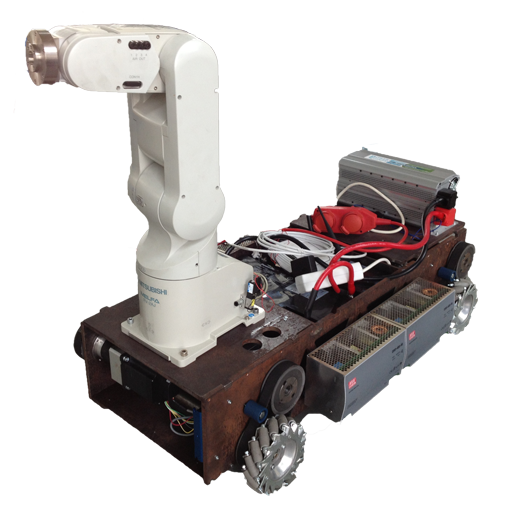
\includegraphics[width=.6\textwidth]{Abbildungen/Roboter} 
\caption[Mecanum-Roboter]{Mecanum-Roboter.}
\label{fig:Roboter}
\end{figure}

\section {Mecanum-Roboter}
\label{sec:Mecanum-Roboter}

Der Mecanum-Roboter ist 1000 mm lang. Er ist mit vier Mecanum-Rädern, die im Rechteck angeordnet sind, ausgestattet. Der Radstand beträgt 775 mm und die Spurbreite beträgt 490 mm. Die Räder haben einen Durchmesser von 115 mm und besitzen jeweils 15 Hilfsrollen. Eine detaillierte Beschreibung folgt im Kapitel \ref{sec:Mecanum-Räder}.

Die Anordnung der Mecanum-Räder und deren Technologie ermöglichen dem Mecanum-Roboter eine omnidirektionale Bewegung. Er kann sich ohne mechanische Lenkung aus jeder Position in jede Richtung fortbewegen.

\subsection*{Mecanum-Räder}
\label{sec:Mecanum-Räder}
Das Mecanum Rad wurde 1973 von der schwedischen Firma Mecanum AB entwickelt und bedient unter-schiedliche Anwendungen. Heutige Anwendungsbeispiele sind unter anderem Förderfahrzeuge, fahrerlose Transportfahrzeuge oder Mobilitätshilfe. Auch in der Robotik finden die Allseitenräder immer häufiger Verwendung.
\begin{figure}[H]
\centering
 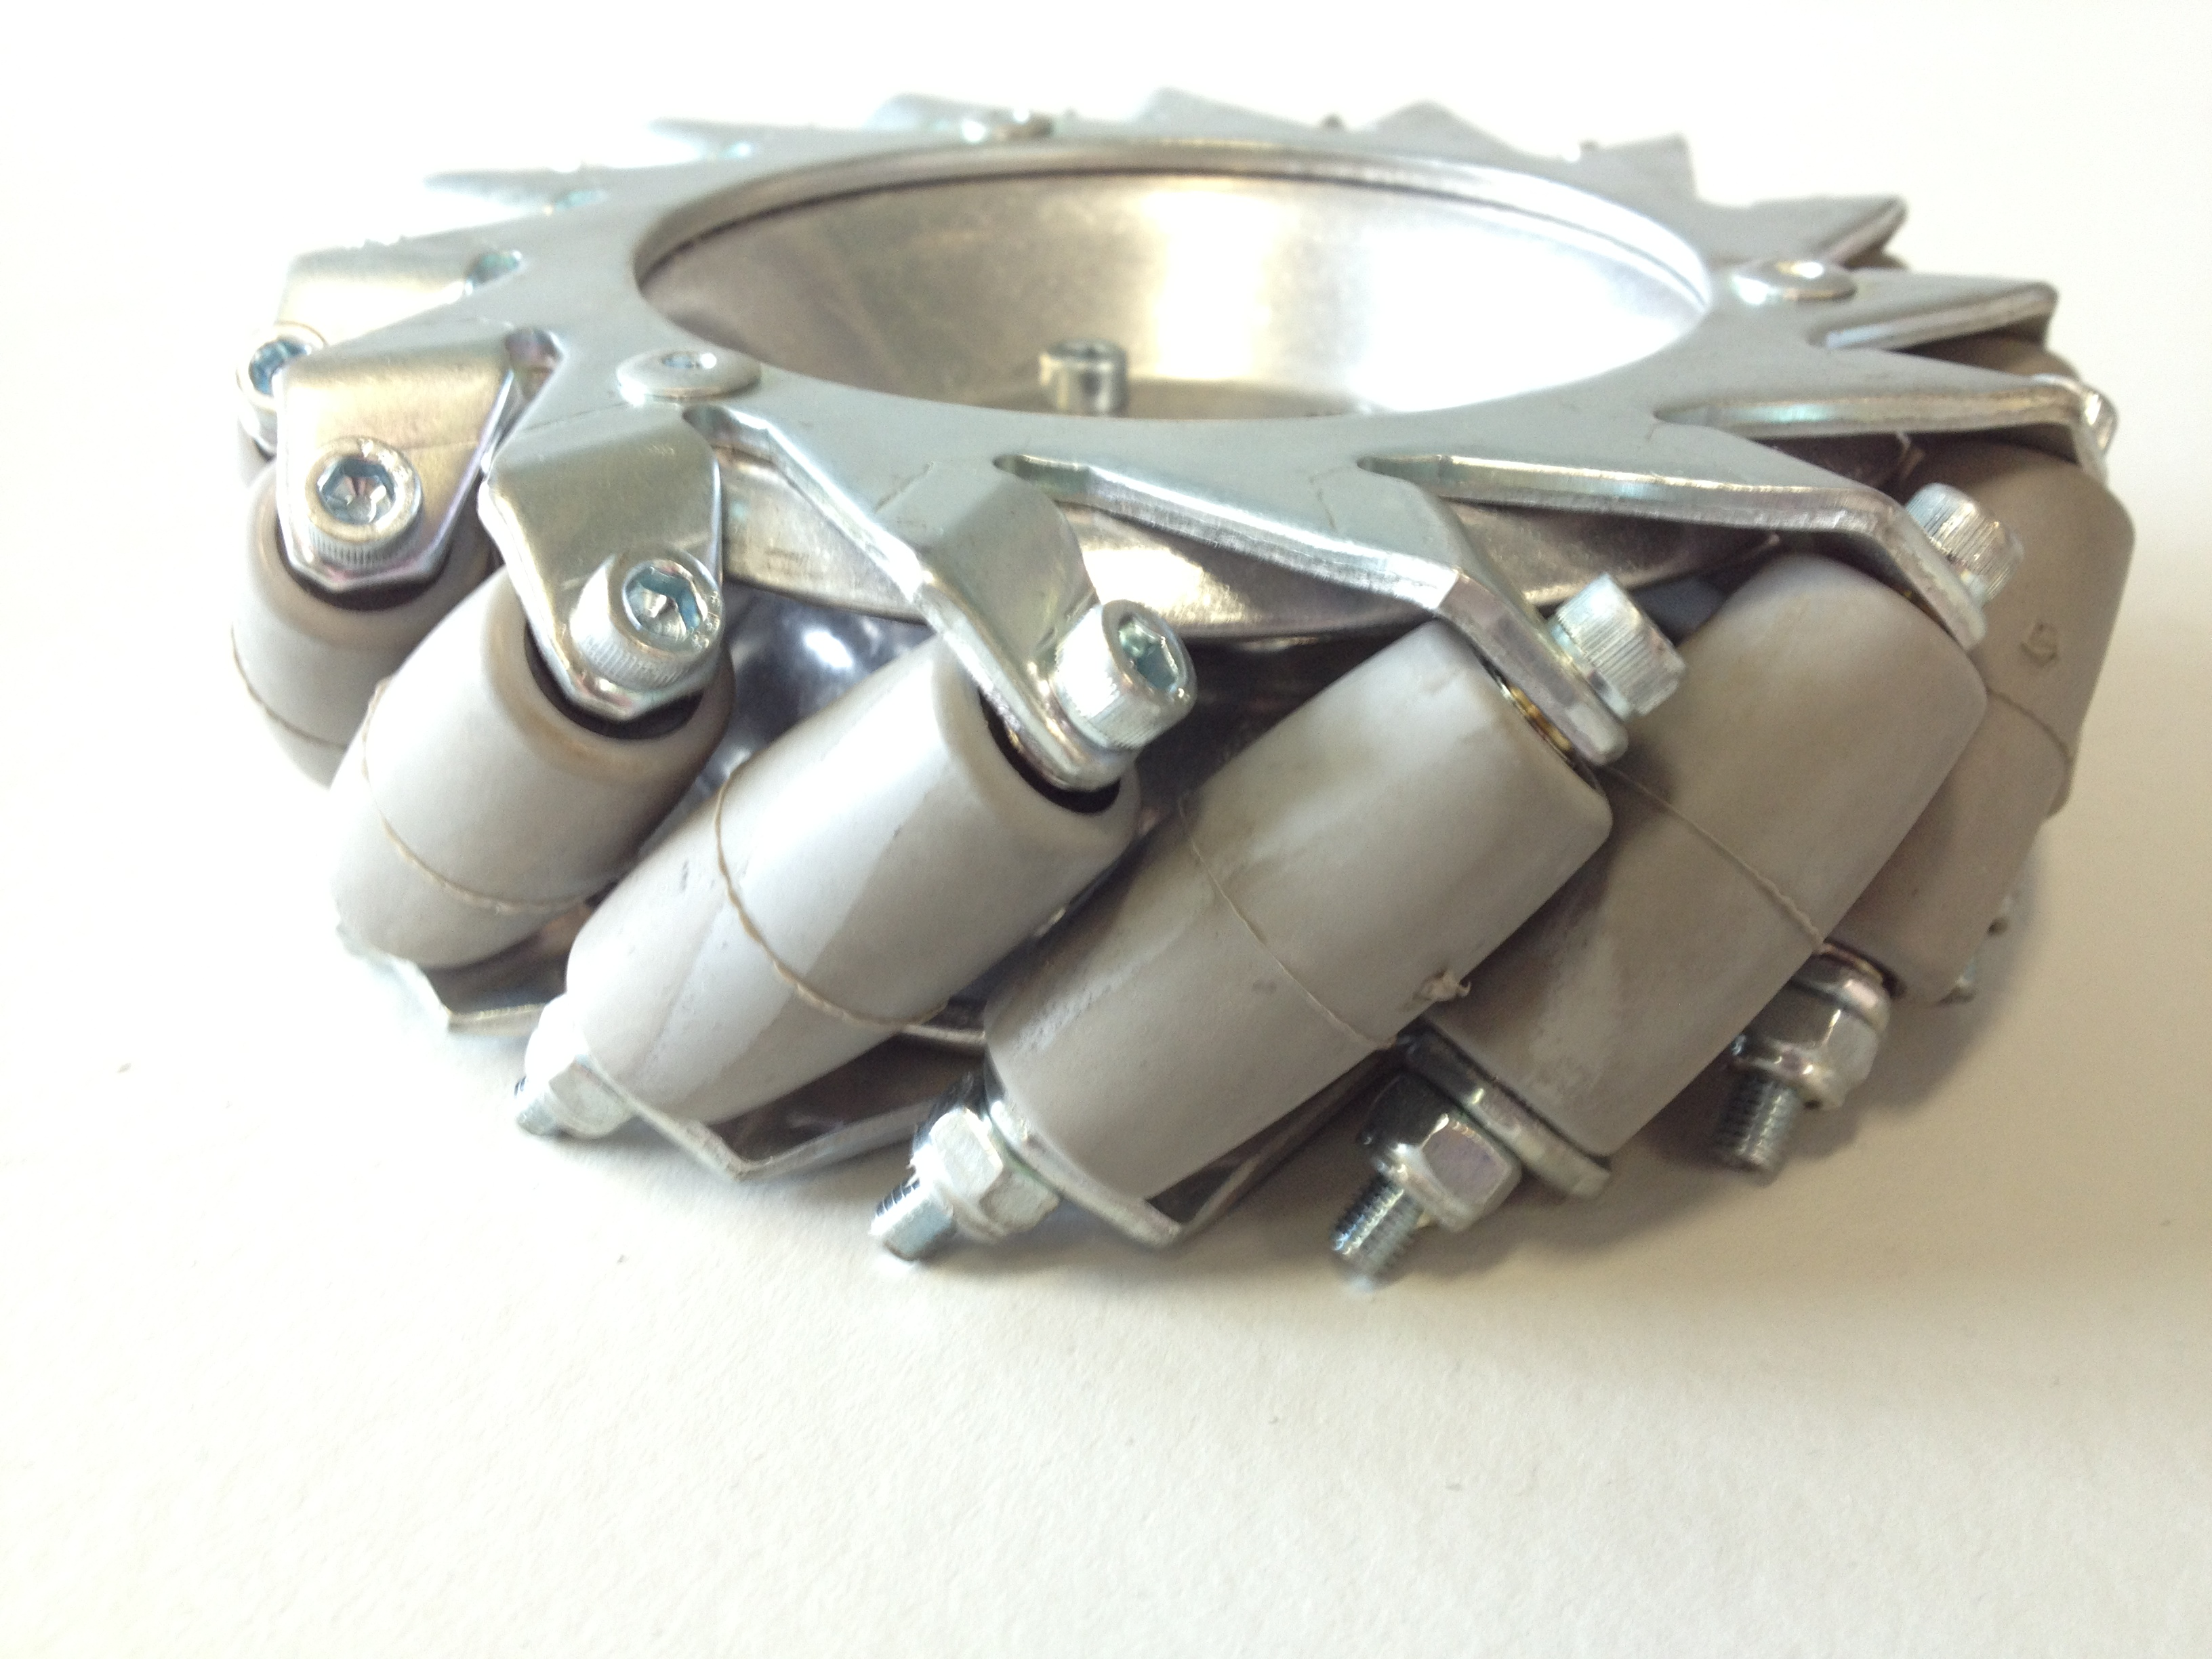
\includegraphics[width=.6\textwidth]{Abbildungen/Mecanumrad} 
\caption[Mecanum-Rad]{Mecanum-Rad.}
\label{fig:Mecanum-Rad}
\end{figure}
Abbilung \ref{fig:Mecanum-Rad} zeigt ein Mecanum-Rad des Mecanum-Roboters. Auf dem Umfang des Rades sind 15 tonnen-förmige beschichtete Rollen im Winkel von 45 Grad zu Radachse angebracht. Diese Rollen haben keinen eigenen Antrieb und sind frei drehbar gelagert. Ausschließlich die Rollen haben Kontakt zum Boden.
Jedes Mecanum-Rad wird von einem Schrittmotor angetrieben. Somit sind Drehsinn und Drehzahl für jedes Rad einzeln ansteuerbar. Dieses ist entscheidend für die omnidirektionale Bewegung.
Durch eine individuelle Drehrichtungsauswahl entstehen durch die Hilfsrollen am Untergrund Kraftvektoren in unterschiedliche Richtungen. Die Summe der Vektoren aller Räder bildet die Gesamtbewegungs-richtung oder auch ein Gesamtdrehmoment.